\documentclass[11pt,reqno]{proc}
\pagestyle{plain}
\usepackage{pgf, tikz}
\usetikzlibrary{arrows, automata}
\usepackage{enumerate}
\usepackage{enumitem}
\usepackage{algorithm}
\usepackage{algorithmic}
%\renewcommand{\thefootnote}{{}}
\newtheorem{theorem}{Theorem}
\newtheorem{lemma}{Lemma}
\newtheorem{corollary}{Corollary}
\newtheorem{proposition}{Proposition}
\newtheorem{definition}{Definition}
\newtheorem{remark}{Remark}
\newtheorem{convention}{Convention}
\newtheorem{sublemma}{Sublemma}
\begin{document}
\title{Mitigating Polarization via Strategic News Exposure} 

\maketitle
\noindent {\bf Introduction} 

The question we plan to address throughout this project is how a recommendation algorithm can choose articles/political media such that after interacting with these new sources, a user’s opinion is as depolarized as possible. We plan to simulate these interactions by generating imaginary people and articles that will interact according to the model explained below. We are using a trust and opinion update rule from one of the relevant papers we have read, linked here, but we have adjusted these equations to better fit our model. Each person generated in our simulation will have a randomly generated initial opinion value (x0) between 0 and 1, an opinion value of 0 indicates a very far left political stance and an opinion of 1 indicates a very far right stance. Additionally, a person has an empathy (h) value that will remain constant throughout the process, as we take this value to be inherent. At this point in our simulation process, we are randomly generating this value for empathy, however we plan to do further research on this topic to make empathy assignments a distribution dependent on the person’s initial opinion value. Although we have not decided this element yet, we have seen some notions in previous work indicating that people with polarized opinions have smaller empathy and people with more left wing views tend to have slightly higher empathy levels. Furthermore, people in this simulation will also have an “inertia” value (i) that indicates their political involvement, which we have found based on previous work to be indicative of a person’s willingness to change opinions. We currently plan to randomly generate this number unless we find work indicating otherwise. These are all the attributes that people will have in our model, articles will simply have a static value indicating their political bias towards the right or left (a) in between 0 and 1.

\vspace{6mm}
\noindent {\bf Algorithm} \\
\begin{center}
     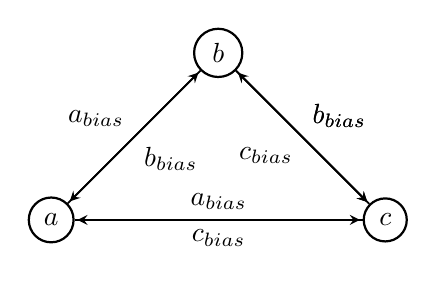
\begin{tikzpicture}[
            > = stealth, % arrow head style
            shorten > = 1pt, % don't touch arrow head to node
            auto,
            node distance = 3cm, % distance between nodes
            semithick % line style
        ]

        \tikzstyle{every state}=[
            draw = black,
            thick,
            fill = white,
            minimum size = 4mm
        ]

        \node[state] (a) {$a$};
        \node[state] (b) [above right of=a] {$b$};
        \node[state] (c) [below right of=b] {$c$};
	\path[->] (a) edge node {$a_{bias}$} (b);
        \path[->] (b) edge node {$b_{bias}$} (c);
        \path[->] (a) edge node {$a_{bias}$} (c);
        	\path[->] (b) edge node {$b_{bias}$} (a);
        \path[->] (b) edge node {$b_{bias}$} (c);
        \path[->] (c) edge node {$c_{bias}$} (a);
        \path[->] (c) edge node {$c_{bias}$} (b);
     \end{tikzpicture}
\end{center}

\begin{algorithm}
\caption{simulatePath(paths, person)}
\begin{algorithmic} 
\STATE $startingStance \leftarrow person.getStance()$
\STATE $finalStances \leftarrow [ ]$
\FOR{path in paths}
\STATE $currentStance \leftarrow startingStance$
\FOR{article in path}
\STATE $currentStance \leftarrow updateStance$$(article.getBias()$, $currentStance, person)$
\ENDFOR
\STATE $finalStances.append(\{currentStance, path\})$
\ENDFOR
\RETURN $minStance(finalStances)$
\end{algorithmic}
\end{algorithm}

To simulate the process of an individual reading a series of articles, we will be using a complete graph. The use of a complete graph implies the idea that a person can read any other article after reading an an article. So in the example above, when a person reads $a$, they can then either read article $b$ or $c$. The complete graph is bidirectional, so when taking the path from article $a$ to article $b$, the weight on the edge is article $a$'s bias and when going from article $b$ to article $a$, the weight on the edge is article $b$'s bias. The weight on the edge is representative of the influence the article will have on the person where the level of influence is dependent on the update function defined above. The goal using this graph is to find a path such that the person's polarization will be mitigated. 

Given a set of possible paths a person can take, we can find the final political stance of the person using this algorithm below. For each path in paths, there will be a set of articles $A = \{$ articles in path $\}$ that the person will read. We will have the person read each article $a_i \in A$, where $i...A.length$, sequentially in the path and update the person's political stance using the update function. Then after calculating the final stance for every path, we will find the most moderate stance and its respective path of articles $A$ which is what we will return. 

\vspace{6mm}
\end{document}